%\documentclass{article}
%\usepackage[utf8]{inputenc}

%\title{Frontmatter}
%\author{wcc.weichihchen }
%\date{May 2021}

%\begin{document}

%\maketitle


%\end{document}



\documentclass[12pt,letterpaper,oneside,draft]{book}
\usepackage[tmargin=1in,bmargin=1in,lmargin=1.5in,rmargin=1in,footskip=0.25in]{geometry}


\usepackage{lipsum}
\usepackage{amsmath}

\usepackage{fancyhdr}
\pagestyle{fancy}
\fancyhf{}
\fancyheadoffset{0cm}
\renewcommand{\headrulewidth}{0pt} 
\renewcommand{\footrulewidth}{0pt}


\usepackage{setspace}
\doublespacing

% For table of contents %

% Redefinition of ToC command to get centered heading
\usepackage{tocloft}
\renewcommand{\cftdotsep}{1}
\renewcommand{\contentsname}{\hspace*{\fill} {TABLE OF CONTENTS} \hspace*{\fill}}
%\renewcommand{\contentsname}{\hfill { } \hfill}
\renewcommand{\cfttoctitlefont}{\mdseries}
\renewcommand{\cftbeforetoctitleskip}{-72pt}
\renewcommand{\cftaftertoctitleskip}{52pt} 
%\renewcommand{\cftchapfont}{}
\renewcommand{\cftpartfont}{\normalfont}
\renewcommand{\cftpartpagefont}{\normalfont}
\renewcommand{\cftchapfont}{\normalfont}
\renewcommand{\cftchappagefont}{\normalfont}

\renewcommand{\cftsecfont}{\normalfont}
\renewcommand{\cftsecpagefont}{\normalfont}

\renewcommand{\cftsubsecfont}{\normalfont}
\renewcommand{\cftsubsecpagefont}{\normalfont}

\renewcommand{\cftpartleader}{\cftdotfill{\cftdotsep}} % dots for parts
\renewcommand{\cftchapleader}{\cftdotfill{\cftdotsep}} % dots for chapters
\renewcommand\cftpartafterpnum{\vspace{-24pt}}

%%%%%%%%%% LIST OF TABLES %%%%%%%%%%
\renewcommand{\listtablename}{\hfill LIST OF TABLES \hfill} 

\renewcommand\cftlottitlefont{\mdseries}
\renewcommand\cfttabfont{\normalfont}
\renewcommand\cfttabpagefont{\normalfont}


\renewcommand{\cftlottitlefont}{{~}\hfill\normalfont}
\renewcommand{\cftafterlottitle}{%
\hfill{~}\\[\baselineskip]{\vspace{-36pt}\normalfont\textit{
Table}}\hspace{372pt}{\normalfont\textit{ Page}}}


\setlength{\cftafterlottitleskip}{40pt}
\setlength{\cfttabindent}{8pt}


%%%%%%%%%% LIST OF FIGURES %%%%%%%%%%
\renewcommand{\listfigurename}{\hfill LIST OF FIGURES \hfill}

\renewcommand\cftloftitlefont{\mdseries}
\renewcommand\cftfigfont{\normalfont}
\renewcommand\cftfigpagefont{\normalfont}


\renewcommand{\cftloftitlefont}{{~}\hfill\normalfont}
\renewcommand{\cftafterloftitle}{%
\hfill{~}\\[\baselineskip]{\vspace{-36pt}\normalfont\textit{
Figure}}\hspace{368pt}{\normalfont\textit{ Page}}}
\setlength{\cftafterloftitleskip}{40pt}
\setlength{\cftfigindent}{8pt}

%%%%%%%%%% LIST OF ABBREVIATIONS %%%%%%%%%%
%\usepackage[nopostdot,style=longtable,nonumberlist]{glossaries}


%\loadglsentries{abbreviations.tex}
%\makeglossaries
%%%%%%%%%% REFERENCES %%%%%%%%%%

\usepackage{natbib}

\setlength\bibsep{12pt}
\newcommand\mybibname{\hfill { } \hfill}
\renewcommand\bibsection{%
    \setlength\bibhang{2in}
    \noindent\normalsize\MakeUppercase{\mybibname}%
    \markboth{\MakeUppercase{\mybibname}}{\MakeUppercase{\mybibname}}%
  }


%%%%%%%%%%%%%%%%%%%%%%%%%%%%%%%%
%%%%%%%%%%%%%%%%%%%%%%%%%%%%%%%%
%%%%%%%%%%%%%%%%%%%%%%%%%%%%%%%%
\usepackage{gensymb}

\usepackage[final]{graphicx}% Include figure files
%\usepackage{graphicx}% Include figure files
\usepackage{hyperref}% add hypertext capabilities
\usepackage[font=normal,format=plain,labelfont=bf,up,textfont=normal,up]{caption} % for the alignment of caption


\begin{document}
	\newgeometry{tmargin=2in,bmargin=1in,lmargin=1.5in,rmargin=1in}
	% Cover
	\frontmatter
    \begin{singlespace}
	{\centering
		YOUR DISSERTATION TOPIC\par
	}
	\vskip 72pt
	{\centering
		by \par
	}
	\vskip 12pt
	{\centering
		YOUR NAME
	\par
	}
	\vskip 24pt
	{\centering
		NAME1, COMMITTEE CHAIR
	\par
	}

	{\centering
		NAME2
	\par
	}
	{\centering
		NAME3
	\par
	}
	{\centering
		NAME4
	\par
	}
	{\centering
		NAME5
	\par
	}
	%\vspace{2.4in}%{180pt}%{2.5in}
	\vspace{204pt}%{2.5in}
	{\centering
		A DISSERTATION
	\par
	}
	\vskip 12pt
	{\centering
		Submitted to the graduate faculty of The University of Alabama at Birmingham,\\
		in partial fulfillment of the requirements for the degree of\\ 
		Doctor of Philosophy
	\par
	}
	\vskip 12pt
	{\centering
		BIRMINGHAM, ALABAMA
	\par
	}
	\vskip 12pt		
	{\centering
		2021
	\par
	}
    \end{singlespace}
    
	% Copyright

	\newgeometry{tmargin=680pt,bmargin=1in,lmargin=1.5in,rmargin=1in}

    \begin{singlespace}
	{\centering
		Copyright by\\
		Wei-Chih Chen\\
		2021\par
	}
    \end{singlespace}
	\restoregeometry
	% Abstract
	\addcontentsline{toc}{part}{ABSTRACT} 
	\pagestyle{plain} % this line would give you
	                      % small roman numeral page number
		{\centering
		\singlespacing
			YOUR DISSERTATION TOPIC\par
		}
		\vskip 12pt
		{\centering
			YOUR NAME\par
		}
		\vskip 12pt
		{\centering
			PHYSICS\par
		}
		\vskip 12pt
		{\centering
			ABSTRACT\par
		}
		\vskip 12pt
%%%%%%%%%% ABSTRACT %%%%%%%%%%
        \lipsum[3-4]

		
		
		\pagebreak
	% Dedication
	\addcontentsline{toc}{part}{DEDICATION} 
	\newgeometry{tmargin=2in,bmargin=1in,lmargin=1.5in,rmargin=1in}
		{\centering
		\singlespacing
			DEDICATION\par
		}
		\vskip 3in
		{\centering
		
		    \textit{For my family}
		    
		}
		\restoregeometry
		
	% Acknowledgement
	\addcontentsline{toc}{part}{ACKNOWLEDGEMENT}
	\newgeometry{tmargin=2in,bmargin=1in,lmargin=1.5in,rmargin=1in}
		{\centering
		\singlespacing
			ACKNOWLEDGEMENT\par
		}
		\vskip 48pt
%%%%%%%%% ACKNOWLEDGEMENT %%%%%%%%%%
        \lipsum[3-4]
    \restoregeometry
    \pagebreak
	
	%%%%%%%%%% TABLE OF CONTENTS PAGE %%%%%%%%%%
	
	{\centering
		\vspace{0pt} \hspace{0pt} \par
	}
	{\centering
		\vspace{1in} \hspace{0pt} \par
	}
	\hspace*{\fill} \textit{Page}



    \tableofcontents
	\pagebreak

	%%%%%%%%%% LIST OF TABLES PAGE %%%%%%%%%%
    
    \addcontentsline{toc}{part}{LIST OF TABLES}
    \listoftables
    \pagebreak
	%%%%%%%%%% LIST OF FIGURES PAGE %%%%%%%%%%

    \addcontentsline{toc}{part}{LIST OF FIGURES}
    \listoffigures
    \pagebreak
	%%%%%%%%%% LIST OF ABBREVIATIONS PAGE %%%%%%%%%%
%    \printglossary[type=\acronymtype,nonumberlist,title=\normalfont \normalsize \protect\centering LIST OF ABBREVIATIONS]
    
    %\printglossary[type=main]
%    \addcontentsline{toc}{part}{LIST OF ABBREVIATIONS}
%    \pagebreak
    

%    \restoregeometry
%    \addtocontents{toc}{\protect\renewcommand{\protect\cftsecleader}{\hfill}}

%%%%%%%%%%%%%%%%%%%%%%%%%%%%%%%%%%%%%%%%%%%%%%%%%%
%%%%%%%%%%%%%%%%%%%%%%%%%%%%%%%%%%%%%%%%%%%%%%%%%%

    \cftaddtitleline{toc}{chap}{\vspace{26pt}CHAPTER\vspace{-16pt}}{}
    

%%%%%%%%%%%%%%%%%%%%%%%%%%%%%%%%%%%%%%%%%%%%%%%%%%
%%%%%%%%%%%%%%%% main text starts %%%%%%%%%%%%%%%%
%%%%%%%%%%%%%%%%%%%%%%%%%%%%%%%%%%%%%%%%%%%%%%%%%%

	\mainmatter 
	%\fancyhead[R]{\thepage}
	\pagestyle{plain}{
		\fancyhf{}
		\fancyhead[R]{\thepage}
	}
	

    %\chapter{1 INTRODUCTION}
    \newcounter{numch}  % counter for chapter
    \addtocounter{numch}{1}
    
    \addcontentsline{toc}{chapter}{\hspace{4pt}  \the\value{numch} \hspace{4pt} INTRODUCTION}
    
	{\centering
		\vspace{0pt} \hspace{0pt} \par
	}
	{\centering
		\vspace{56pt} CHAPTER  \the\value{numch}
	}
	{\centering\singlespacing
		INTRODUCTION
	    \par
	}
	{\centering
		\vspace{0pt} \hspace{0pt} \par
	}
    \lipsum[1-5]
    
    %\subsection*{Summary of Superhard Materials}
    \addcontentsline{toc}{subsection}{subtopic 1}
	{\centering
		\vspace{12pt}subtopic 1
	    \par
	}

\lipsum[2-4]
	\begin{equation}
		\begin{aligned}
		\label{eq}
			H_V = 1854.4\frac{F}{d^2}.
		\end{aligned}
	\end{equation}
\lipsum[2-4]

\lipsum[2-4]
    
    \begin{figure}[t]
        \centering
        \captionsetup{singlelinecheck = false, justification=justified}
        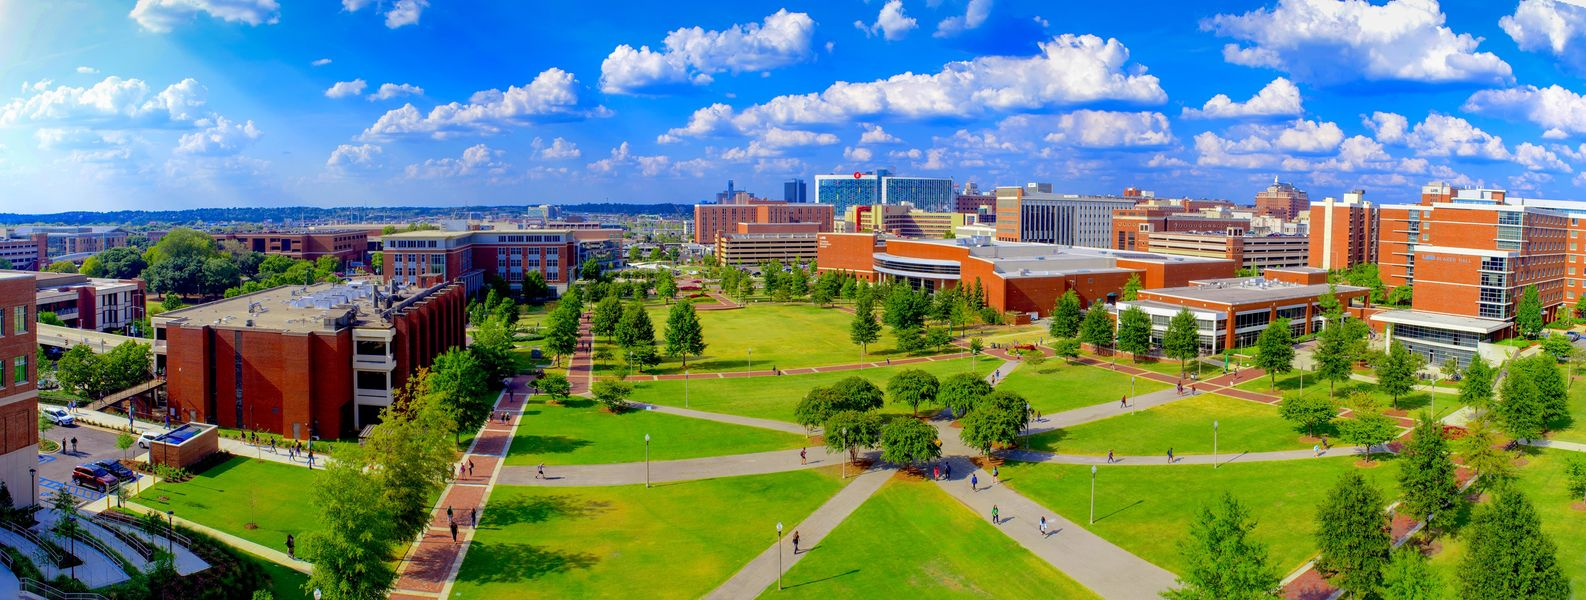
\includegraphics[width=0.95\textwidth]{UAB_Campus_Green.jpg}
        \caption[caption in contents of figures]{This is the caption for Figure 1.}
        \label{fig:1}
    \end{figure}
    
\lipsum[2-4]




\vspace{24pt}


	\setlength{\tabcolsep}{12pt} % Default value: 6pt
	\renewcommand{\arraystretch}{1.5} % Default value: 1
    \begin{table}[htb]
    \captionsetup{singlelinecheck = false, justification=justified}
    %\centering
    \caption[caption in contents of tables]{This is the caption for the table.}
    \label{tab:1}
    \begin{tabular*}{\textwidth}{c|c|c|c}
        Borides  & {$H_V$ (GPa) @ 0.49 N load} & $H_V$ (GPa) @ high load & Reference  \\ \hline
        %c-BN      &       & 65 @ 4.9N   & ~\cite{cBN_65_GPa_liu2019hardness} \\
        CrB       &  30   & 20 @ 4.9 N   & ~\cite{CrB_han2015hardness} \\
        WB        &  35   & 18 @ 4.9 N   &
        ~\cite{WB_yeung2016superhard} \\
        WB$_2$    &  30   & 22 @ 4.9 N   &
        ~\cite{pangilinan2018superhard} \\
        TiB$_2$   &  -    & 20 @ 5.0 N   & ~\cite{TiB2_munro2000material} \\
        ZrB$_2$   &  -    & 17 @ 9.8 N   & ~\cite{ZrB2_HfB2_zapata2013mechanical} \\
        HfB$_2$   &  -    & 20 @ 9.8 N   & ~\cite{ZrB2_HfB2_zapata2013mechanical} \\
        CrB$_2$   &  -    & 16 @ 4.9 N   & ~\cite{CrB2_CrB4_wang2014crystal} \\
        WB$_4$    &  43   & 28 @ 4.9 N   & ~\cite{WB4_mohammadi2011tungsten} \\
        CrB$_4$   &  44   & 30 @ 4.9 N   & ~\cite{CrB2_CrB4_wang2014crystal} \\  
        %CaB$_6$   &  26   & 24 @ 4.9N   & ~\cite{CaB6_xin2011properties} \\  
        ZrB$_{12}$&  42, 40   & 28, 27 @ 4.9 N   & ~\cite{YB12_akopov2019synthesis, ZrB12_ma2017ultrastrong} \\
        YB$_{12}$ &  38   & 26 @ 4.9 N   & ~\cite{YB12_akopov2019synthesis} \\
    \end{tabular*}
    \end{table}

\vspace{24pt}

\lipsum[2-4]


\pagebreak
























    %\subsection*{Topological Materials}
    \addcontentsline{toc}{subsection}{subtopic 2}
	{\centering
		\vspace{12pt} subtopic 2
	    \par
	}
\lipsum[2-4]





	
    \pagebreak
    
	
    %\subsection*{Overview of Remaining Chapters}
    \addcontentsline{toc}{subsection}{subtopic 3}
	{\centering
		\vspace{12pt} subtopic 3
	    \par
	}
    \lipsum[2-4]
    


    \clearpage

    %\chapter{2 METHODS}
    \addtocounter{numch}{1}
	\addcontentsline{toc}{chapter}{\hspace{4pt}  \the\value{numch} \hspace{4pt} METHODS}
	{\centering
		\vspace{0pt} \hspace{0pt} \par
	}
	{\centering
		\vspace{56pt} CHAPTER  \the\value{numch}
	}
	{\centering\singlespacing
		METHODS
	    \par
	}
	{\centering
		\vspace{0pt} \hspace{0pt} \par
	}

    %\subsection*{Density Functional Theory}
    \addcontentsline{toc}{subsection}{subtopic 1}
	{\centering
		\vspace{12pt} subtopic 1
	    \par
	}
\lipsum[2-4]
\pagebreak






    %\subsection*{Evolutionary Algorithm}
    \addcontentsline{toc}{subsection}{subtopic 2}
	{\centering
		\vspace{12pt} subtopic 2
	    \par
	}
\lipsum[2-4]
\pagebreak
    
    %\chapter{3 MACHINE LEARNING AND EVOLUTIONARY DISCOVERY OF TERNARY SUPERHARD MATERIALS}
    \addtocounter{numch}{1}
	\addcontentsline{toc}{chapter}{\hspace{0pt}  \the\value{numch} \hspace{4pt} RESULTS}
	{\centering
		\vspace{0pt} \hspace{0pt} \par
	}
	{\centering
		\vspace{56pt} CHAPTER  \the\value{numch}
	}
	{\centering\singlespacing
		RESULTS
	    \par
	}
	{\centering
		\vspace{0pt} \hspace{0pt} \par
	}
	
	
	
	
	
    %\subsection*{B-C-N Superhard Materials}
    \addcontentsline{toc}{subsection}{subtopic 1}
	{\centering
		\vspace{12pt} subtopic 1 
	    \par
	}

\lipsum[2-4]
\pagebreak




		

			
	
    
    \pagebreak
    %\subsection*{B-N-O Superhard Materials}
    \addcontentsline{toc}{subsection}{subtopic 2}
	{\centering
		\vspace{12pt} subtopic 2
	    \par
	}
\lipsum[2-4]
\pagebreak

    
    \pagebreak

    
    %\chapter{4 STRUCTURAL AND TOPOLOGICAL PHASE TRANSITIONS IN TOPOLOGICAL QUANTUM MATERIALS}
    \addtocounter{numch}{1}
	\addcontentsline{toc}{chapter}{\hspace{0pt}  \the\value{numch} \hspace{4pt} DISCUSSION}
	{\centering
		\vspace{0pt} \hspace{0pt} \par
	}
	{\centering
		\vspace{56pt} CHAPTER  \the\value{numch}
	}
	{\centering\singlespacing
		DISCUSSION
	    \par
	}
	{\centering
		\vspace{0pt} \hspace{0pt} \par
	}
	

    
    %\subsection*{Topological Phase Transition in ZrTe$_5$}
    \addcontentsline{toc}{subsection}{subtopic 1}
	{\centering
		\vspace{12pt} subtopic 1 
	    \par
	}

\lipsum[2-4]
\pagebreak


\pagebreak
    
    %\subsection*{Structrual and Topological Phase Transitions in LaN}
    \addcontentsline{toc}{subsection}{subtopic 2}
	{\centering
		\vspace{12pt} subtopic 2
	    \par
	}

\lipsum[2-4]
\pagebreak




    

	

    %\chapter{5 CONCLUSION}
    \addtocounter{numch}{1}
    \addcontentsline{toc}{chapter}{\hspace{4pt}  \the\value{numch} \hspace{4pt} CONCLUSION}
	
	{\centering
		\vspace{0pt} \hspace{0pt} \par
	}
	{\centering
		\vspace{56pt} CHAPTER  \the\value{numch}
	}
	{\centering\singlespacing
		CONCLUSION
	    \par
	}
	{\centering
		\vspace{0pt} \hspace{0pt} \par
	}
	

	
\lipsum[2-4]
\pagebreak
	
    % List of Publications

    \addcontentsline{toc}{chapter}{LIST OF PUBLICATIONS}
	
	{\centering
		\vspace{0pt} \hspace{0pt} \par
	}
	{\centering
		\vspace{56pt} LIST OF PUBLICATIONS
	}
	{\centering\singlespacing
		
	    \par
	}
	{\centering
		\vspace{0pt} \hspace{0pt} \par
	}
	\noindent Wei-Chih Chen, Joanna N. Schmidt, Da Yan, Yogesh K. Vohra, and Cheng-Chien Chen, “Machine Learning and Evolutionary Prediction of Superhard B-C-N Compounds”, {\it npj Comput Mater} {\bf 7}, 114 (2021).
	
	\vspace{12pt}

    \noindent Wei-Chih Chen, Chia-Min Lin, Joseph Maciejko, and Cheng-Chien Chen, “Structural and Topological Phase Transitions in LaN Driven by Pressure and temperature”, arXiv:2104.12879 (2021).

	\vspace{12pt}

	
	\pagebreak

	{\centering
		\vspace{0pt} \hspace{0pt} \par
	}
	{\centering
		\vspace{24pt} \hspace{0pt} \par
	}
	\hfill  REFERENCES { } { } \hfill
	{\centering
		\vspace{0.2in} \hspace{0pt} \par
	}
	
    \addcontentsline{toc}{chapter}{REFERENCES}
    \bibliographystyle{unsrt}
%    \bibliographystyle{phys}
%    \bibliographystyle{abbrv}
    \bibliography{bibfile.bib}

    %\pagebreak
    %for testing: \gls{HV}
\end{document}
